% !TEX root = main.tex
\documentclass[10pt, a4paper]{article}

% ── Packages ──────────────────────────────────────────────────────────────────
\usepackage[
  top=0.35in, bottom=0.35in,
  left=0.45in, right=0.45in
]{geometry}
\usepackage[dvipsnames]{xcolor}
\usepackage{hyperref}
\usepackage{graphicx}
\usepackage{titlesec}
\usepackage{enumitem}
\usepackage{array}
\usepackage{tabularx}
\usepackage{parskip}

% ── Hyperlink styling ─────────────────────────────────────────────────────────
\hypersetup{
  colorlinks=true,
  urlcolor=black,
  linkcolor=black
}

\pagestyle{empty}

% Section formatting
\titleformat{\section}
  {\normalsize\bfseries}
  {}{0em}{\MakeUppercase}
  [\vspace{-6pt}\rule{\linewidth}{0.5pt}]

\titlespacing{\section}{0pt}{6pt}{2pt}

<<<<<<< HEAD
\setlist[itemize]{noitemsep, topsep=0pt, partopsep=0pt, parsep=0pt, leftmargin=1.2em, itemsep=0pt}
=======
\setlist[itemize]{noitemsep, topsep=0pt, partopsep=0pt, parsep=0pt, leftmargin=1.1em, itemsep=0pt}
>>>>>>> main

\setlength{\parindent}{0pt}
\setlength{\parskip}{0pt}

% Set base font size slightly larger than 10pt default
\fontsize{10.5}{13.5}\selectfont

% ══════════════════════════════════════════════════════════════════════════════
\begin{document}

% ── HEADER ────────────────────────────────────────────────────────────────────
\noindent
\begin{minipage}[c]{0.48\textwidth}
  \raggedright
  {\fontsize{24}{28}\selectfont \textbf{YOUR NAME}}\par
<<<<<<< HEAD
  \vspace{5pt}
  {\large\itshape\color{gray} Computer Science Engineer}\par
=======
  \vspace{3pt}
  {\large\itshape\color{gray} Backend Engineer $|$ API \& Scalable Systems}\par
>>>>>>> main
\end{minipage}%
\hfill
\begin{minipage}[c]{0.36\textwidth}
  \raggedleft
  \begin{minipage}[c]{0.68\linewidth}
    \raggedleft
    {\small\itshape\color{gray}
      \href{mailto:your.email@example.com}{your.email@example.com}\\[3pt]
      +91\,00000\,85302\\[3pt]
      \href{https://linkedin.com/in/your-linkedin}{linkedin.com/in/your-linkedin}\\[3pt]
      \href{https://github.com/your-github}{github.com/your-github}\\
    }
  \end{minipage}%
  \hspace{0.1pt}
\begin{minipage}[c]{0.26\linewidth}
    \raggedleft
    \fboxsep=2pt\fboxrule=0.5pt
    \fbox{%
      \IfFileExists{../assets/profile-photo.jpg}{%
        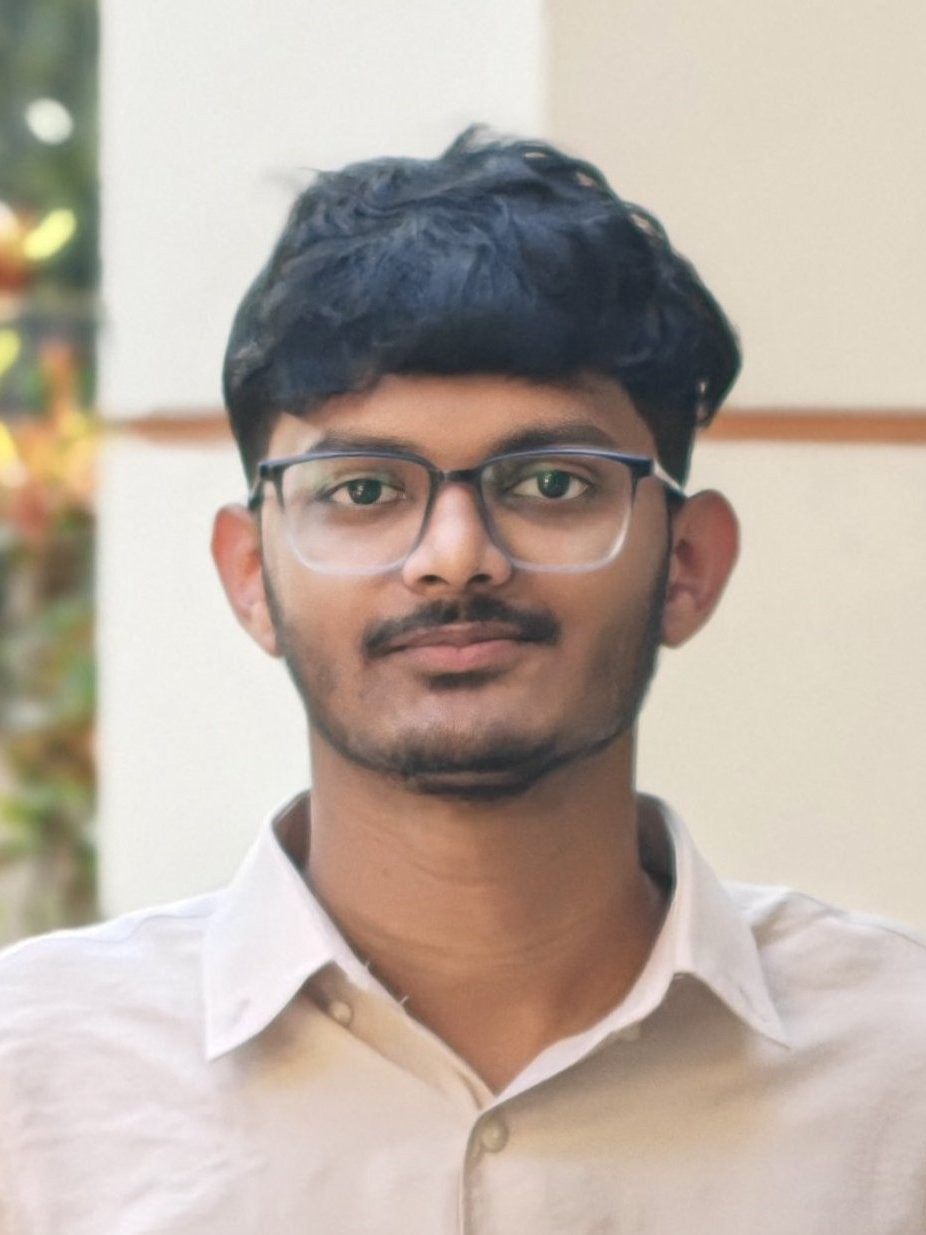
\includegraphics[height=0.75in,keepaspectratio]{../assets/profile-photo.jpg}}{%
      \IfFileExists{../assets/profile-photo.png}{%
        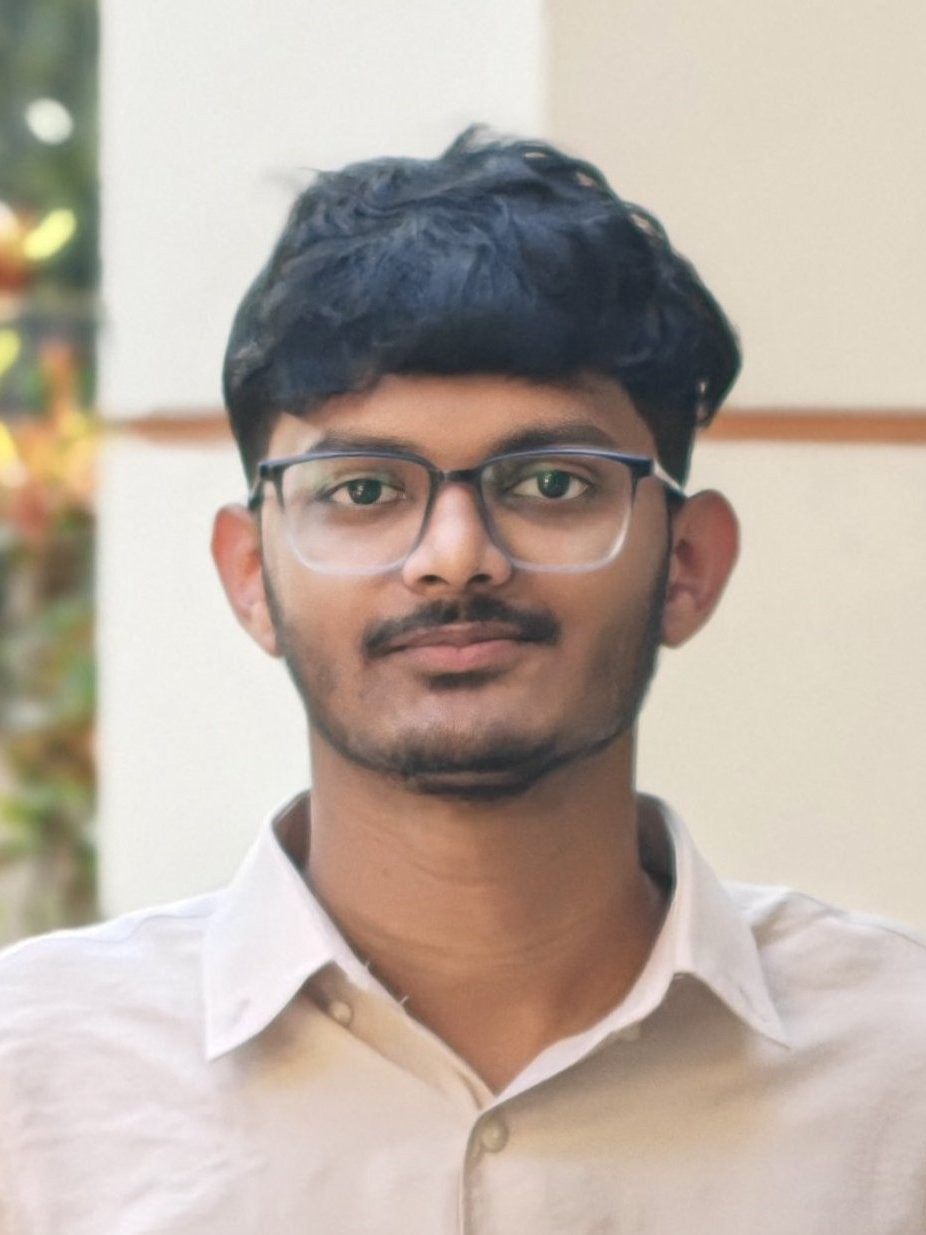
\includegraphics[height=0.75in,keepaspectratio]{../assets/profile-photo.png}}{%
      \IfFileExists{../assets/photo.jpg}{%
        \includegraphics[height=0.75in,keepaspectratio]{../assets/photo.jpg}}{%
      \IfFileExists{../assets/photo.png}{%
        \includegraphics[height=0.75in,keepaspectratio]{../assets/photo.png}}{}}}}%
    }%
  \end{minipage}
\end{minipage}

<<<<<<< HEAD

% ── YOUR RESUME CONTENT GOES BELOW ───────────────────────────────────────────
\section*{Objective}

Developer with hands-on experience in backend systems, REST APIs, and cloud deployment. Skilled in Python, JavaScript, Go, and Rust across web, desktop, and computer vision projects.
=======
% ── CONTENT ──────────────────────────────────────────────────────────────────
\section*{Professional Summary}

Backend Engineer building scalable, real-time backend processing systems with Python, Node.js, and Go. Active GitHub developer focused on high-performance architectures and event-driven automation pipelines. Optimized system efficiency by over 40\% while delivering production-ready technical solutions.
>>>>>>> main

%------------------------------------------------------------
% TECHNICAL SKILLS
%------------------------------------------------------------
\section*{Skills}

<<<<<<< HEAD
\renewcommand{\arraystretch}{1.05}
\begin{tabular}{@{} >{\bfseries}p{3.8cm} p{13cm} @{}}
Languages           & Python, Java, C, JavaScript, Go, Rust \\
Web Development     & HTML, CSS, React.js, Node.js, Next.js, PHP \\
Frameworks          & Flask, Django, Express.js, Tauri, Wails, Flutter, Firebase \\
Databases           & MongoDB, MySQL, Supabase \\
Developer Tools     & Git, GitHub, Docker, Postman, REST APIs \\
Deployment          & Netlify, Vercel, Render, DigitalOcean, Cloudflare, Heroku \\
Operating Systems   & Linux, Windows \\
=======
\renewcommand{\arraystretch}{1.0}
\begin{tabular}{@{} >{\bfseries}p{3.8cm} p{13cm} @{}}
Languages           & Python, Go, JavaScript \\
Backend             & Node.js, Flask, Django, Express.js, REST API Design, Microservices \\
Databases           & MongoDB, MySQL, Supabase, DB Optimization \\
Cloud/Deployment    & AWS (API Gateway), Docker, DigitalOcean, Vercel, Render \\
Architecture        & Scalable Architecture, Authentication, Batch Processing \\
>>>>>>> main
\end{tabular}

%------------------------------------------------------------
% PROJECTS
%------------------------------------------------------------
\section*{Projects}

<<<<<<< HEAD
\textbf{AI-Based Smart Traffic System Using Computer Vision} \hfill \textit{Python, YOLO, Flask \quad Jan 2025}
\begin{itemize}
\item Implemented a YOLO-v8 detection pipeline achieving 92--94\% accuracy across varied traffic conditions.
\item Reduced simulated intersection wait times by 20--25\% via adaptive signal control algorithms.
\item Optimized model inference for real-time edge deployment, maintaining low-latency processing ($<$200ms/frame).
\end{itemize}

\vspace{3pt}

\textbf{Certificate Generator and Verification System} \hfill \textit{Node.js, Firebase, EJS, Tailwind \quad Dec 2024} \quad \href{https://github.com/your-github/advanced-certificate-generator}{[GitHub]}
\begin{itemize}
\item Automated bulk certificate generation for 1,000+ records per batch, reducing manual effort by \textasciitilde85\%.
\item Implemented QR-based verification enabling instant credential validation with minimal manual intervention.
\item Engineered an interactive canvas editor supporting dynamic layouts and reusable template components.
\end{itemize}

\vspace{3pt}

\textbf{IRRIGO -- Smart Irrigation Platform} \hfill \textit{Next.js, Flask, Python, REST APIs \quad Oct 2024}
\begin{itemize}
\item Built an AI-assisted irrigation platform integrating satellite and weather data for improved scheduling decisions.
\item Analyzed 50+ farm scenarios to optimize water usage, reducing estimated wastage by \textasciitilde15--20\%.
\item Engineered a full-stack analytics dashboard for real-time monitoring using RESTful APIs.
\end{itemize}

\vspace{3pt}
=======
\textbf{Certificate Generator and Verification System} \hfill \textit{Node.js, Firebase, EJS, Tailwind \quad Dec 2024} \quad \href{https://github.com/your-github/advanced-certificate-generator}{[GitHub]}
\begin{itemize}
\item Designed scalable REST API for high-throughput bulk certificate processing (1,000+ records) with \textasciitilde85\% effort reduction.
\item Engineered optimized database queries and API endpoints ensuring efficient data retrieval and validation.
\item Implemented secure QR-based verification enabling instant, cryptographically-linked credential validation.
\end{itemize}

\vspace{2pt}

\textbf{IRRIGO -- Smart Irrigation Platform} \hfill \textit{Next.js, Flask, Python, REST APIs \quad Oct 2024}
\begin{itemize}
\item Designed scalable RESTful APIs and data pipelines handling real-time environmental data processing.
\item Built an AI-assisted backend integrating satellite and weather data for autonomous scheduling.
\item Developed efficient resource allocation logic, reducing water wastage by \textasciitilde15--20\%.
\end{itemize}

\vspace{2pt}

\textbf{AI-Based Smart Traffic System Using Computer Vision} \hfill \textit{Python, YOLO, Flask \quad Jan 2025}
\begin{itemize}
\item Integrated computer vision pipeline with event-driven backend decision engine for real-time traffic signal control.
\item Reduced simulated intersection wait times by 20--25\% via adaptive frequency-control algorithms.
\item Engineered model inference for real-time edge deployment, maintaining $<$200ms processing latency.
\end{itemize}

\vspace{2pt}
>>>>>>> main

\textbf{DroidOps -- Android Device Management GUI} \hfill \textit{Tauri, React, Rust, TypeScript \quad Dec 2025} \quad \href{https://github.com/your-github/droidops}{[GitHub]}
\begin{itemize}
\item Built a cross-platform Tauri/Rust ADB GUI, reducing manual device operations by \textasciitilde30--40\%.
<<<<<<< HEAD
\item Streamlined device management via intuitive UI, improving device detection and interaction speed.
\item Integrated batch processing features, reducing repetitive testing cycles and improving developer efficiency.
\end{itemize}

\vspace{3pt}

\textbf{GlyphDeck -- Desktop Font Manager} \hfill \textit{Go, TypeScript, Wails \quad Nov 2025} \quad \href{https://github.com/your-github/GlyphDeck}{[GitHub]}
\begin{itemize}
\item Developed a Go-based font manager indexing 800+ local fonts with optimized search and preview.
\item Enhanced usability and navigation efficiency by \textasciitilde30--40\% through improved UI interactions.
\item Optimized memory usage, delivering a lightweight \textasciitilde25MB executable with native performance.
=======
\item Streamlined device management via intuitive UI with optimized Rust backend command execution.
\item Integrated batch processing features for automated unit testing and environment setup.
\end{itemize}

\vspace{2pt}

\textbf{GlyphDeck -- Desktop Font Manager} \hfill \textit{Go, TypeScript, Wails \quad Nov 2025} \quad \href{https://github.com/your-github/GlyphDeck}{[GitHub]}
\begin{itemize}
\item Developed a Go-based font manager indexing 800+ local fonts with sub-500ms retrieval latency.
\item Enhanced navigation efficiency by \textasciitilde30--40\% through optimized search and retrieval logic.
\item Developed memory-efficient native executable (\textasciitilde25MB) with native performance using Go.
>>>>>>> main
\end{itemize}

%------------------------------------------------------------
% EDUCATION
%------------------------------------------------------------
\section*{Education}

\textbf{B.Tech in Computer Science and Engineering} \hfill \textbf{2022 -- 2026}\\
<<<<<<< HEAD
Mar Baselios Christian College of Engineering and Technology, Kuttikkanam \hfill APJ Abdul Kalam Technological University
=======
Mar Baselios Christian College of Engg. \& Tech., Kuttikkanam \hfill APJ Abdul Kalam Technological University
>>>>>>> main

%------------------------------------------------------------
% CERTIFICATIONS
%------------------------------------------------------------
\section*{Certifications}

<<<<<<< HEAD
\renewcommand{\arraystretch}{1.1}
\begin{tabular}{@{} p{7.8cm} p{6.5cm} p{2.5cm} @{}}
\textbf{Certificate}                  & \textbf{Issuer}              & \textbf{Year} \\[1pt]
Programming with Python               & Python Institute (OpenEDG)   & 2024 \\
Python for Data Science               & NPTEL -- IIT Madras          & 2024 \\
JavaScript Foundations Professional   & Mozilla                      & Jul 2025 \\
=======
\renewcommand{\arraystretch}{1.0}
\begin{tabular}{@{} p{7.8cm} p{6.5cm} p{2.5cm} @{}}
\textbf{Certificate}                  & \textbf{Issuer}              & \textbf{Year} \\[1pt]
Programming with Python               & Python Institute (OpenEDG)   & 2024 \\
>>>>>>> main
Amazon API Gateway for Serverless     & AWS Training                 & Jun 2025 \\
Ubuntu Linux Professional Certificate & Canonical                    & Nov 2025 \\
\end{tabular}

<<<<<<< HEAD
%------------------------------------------------------------
% ACHIEVEMENTS
%------------------------------------------------------------
\section*{Achievements}

\begin{tabular}{@{} p{9.5cm} p{8cm} @{}}
Galactic Problem Solver              & NASA Space Apps Challenge 2024 \\
Global Connection Recognition        & NASA Space Apps Challenge 2025 \\
Global Nominee                       & NASA Space Apps Challenge 2025 \\
\end{tabular}

%------------------------------------------------------------
% INTERESTS & LANGUAGES
%------------------------------------------------------------
\section*{Additional Information}

\begin{tabular}{@{} >{\bfseries}p{3.8cm} p{13cm} @{}}
Areas of Interest & Backend Systems, API Development, Full Stack Development, Desktop Applications, Mobile Applications \\
Languages         & English, Malayalam \\
\end{tabular}

=======
>>>>>>> main
\end{document}